\documentclass[11pt,letterpaper,twoside,english]{article}
\usepackage{fullpage}
\usepackage{babel}

\usepackage{float}
\usepackage{graphicx}
\usepackage[authoryear]{natbib}
\usepackage[unicode=true, pdfusetitle,
 bookmarks=true,bookmarksnumbered=false,bookmarksopen=false,
 breaklinks=false,pdfborder={0 0 0},backref=false,colorlinks=false]
 {hyperref}


\ifx\pdfoutput\undefined
    % we are running LaTeX, not pdflatex

\else
    % we are running pdflatex, so convert .eps files to .pdf

    \usepackage{epstopdf}
\fi

\author{Yizhi Cai \& Chris Lasher\\
Supervised by Prof.~John Jelesko}
\title{GBCB 5874 Final Paper: Jelesko Pathway Evolution Database}
\date{May 11, 2009}

\usepackage{fancyhdr}
\setlength{\headheight}{15pt}
\pagestyle{fancy}

\lhead{GBCB 5874 Final Paper}
\rhead{Cai \& Lasher}

\begin{document}
\maketitle

\section{Introduction (Chris Lasher)}

\textit{Disclaimer: Much of the research described in the motivation behind
this work is pending publication. Please exercise discretion in discussing
them with colleagues.}

Through the process of evolution, life has taken diverse forms, made possible
through a concomitantly diverse range of metabolic capabilities. When examined
across evolutionary time, the vast majority of biological processes display
consistent histories that follow what biologists casually refer to as the
``tree of life''. (See Figure \ref{fig:tree_of_life}.)

\begin{figure}[htbp]
    \begin{center}
        \includegraphics[width=0.65\linewidth]{figures/Phylogenetic_tree_hgt}
    \end{center}
    \caption{A widely recognized representation of the phylogenetic tree
    across all known domains of life. The first split from the last common
    ancestor gave rise to the domain of modern day bacteria. The next split
    came between archaea and eukaryotes. Most phylogenetic analyses for genes
    conserved across domains produce similar trees as this one. Two notable
    exception to the evolutionary history of genes occured as mass horizontal
    gene transfer events in the form of the ancestral origins of the
    mitochondrion, arising from a symbiosis between ancestral
    $\alpha$-proteobacteria and the progenitor to modern eukaryotes
    (illustrated as the horizontal black arrow), and the origins of the
    chloroplast and plant plastids, arising from a symbiosis between ancestral
    cyanobacteria and the progenitor to plants (illustrated as the horizontal
    cyan arrow). \textit{Image modified from public domain work.}}
    \label{fig:tree_of_life}
\end{figure}

Two very notable exceptions to the tree of life came about through two massive
horizontal gene transfer events that gave rise, first, to mitochondria, and
second, to plastids (e.g., chloroplasts). The mechanism for these phenomena is
described by the endosymbiotic hypothesis. Summarized briefly, ancestral
bacteria most closely related to the $\alpha$-proteobacteria engaged in a
tight endosymbiotic relationship with the progenitor to modern day eukaryotes,
living inside the primordial eukaryotic cells. Over time the two became
interdependent, and a large amount of the ancient $\alpha$-proteobacterial
genome was lost or transfered over to the primordial eukaryotic cells' genomes
in very large portions, eventually giving rise to what we now know as modern
mitochondria. Similar events are believed to have led to the creation of
plastids in plants. Keeling and Palmer \cite{keeling_horizontal_2008} provide
an excellent recent review on this topic.

While the origins of mitochondria and plastids provide the most grand examples
of horizontal gene transfer between domains of the tree of life, smaller
events do occur, possibly introducing additional metabolic capabilities to the
receiving host. For recently involved eukaryotes, there is a great gap between
metabolic capabilities; fungi and plants possess fairly broad biochemical
repertoires, while metazoans (animals) have comparatively narrower abilities.
The exact reasons for this divide are still the subject of active research.
While gene loss certainly plays a role, it's becoming increasingly apparent
that introduction of genes via horizontal gene transfer also remains key.

\begin{figure}[tbhp]
    \begin{center}
        \includegraphics[width=0.3\linewidth]{figures/ODC_figure}
        \hspace{0.02\linewidth}
        \includegraphics[width=0.3\linewidth]{figures/ADC_figure}
        \hspace{0.02\linewidth}
        \includegraphics[width=0.3\linewidth]{figures/QPT_figure}
    \end{center}
    \caption{Examples of three different phylogenetic histories for enzymes
    responsible for nicotine biosynthesis. The tree for ornithine
    decarboxylase (ODC, left) illustrates phylogeny to be expected for an
    evolutionary history consistent with that widely accepted for the tree of
    life--the plant sequences (dark green) are most closely associated with
    other eukaryotes (fungi in blue, and metazoans in red). The tree for
    arginine decarboxylase (ADC, center) is consistent with accepted
    horizontal gene transfer that occurred during the incorporation of
    ancestral cyanobacterial (cyan) genetic material that gave rise to the
    modern day chloroplast. The tree for quinolate phosphoribosyl transferase
    (QPT, right) illustrates a much more complex evolutionary history, which
    indicates its most likely origins were from a horizontal gene transfer
    event from CFB bacteria (orange). \textit{Image courtesy of Prof.~John
    Jelesko.}}
    \label{fig:phylo_histories}
\end{figure}

The Jelesko lab encountered such an illustrative case in earlier research on
the origins behind a very important secondary metabolite: nicotine.  Exploring
the evolutionary histories of each enzyme individually, they discovered rather
unexpected results. While evolutionary evidence indicated that some of the
enzymes in the nicotine biosynthesis pathway likely descended from traditional
eukaryotic origins, for five of the seven known enzymes, the closest homolog
resided not with other eukaryotes, but with prokaryotes. (See Figure
\ref{fig:phylo_histories} for examples of the deduced phylogenetic histories.)
Even more interesting was the patchwork history that arose when viewing the
pathway overlayed with the evolutionary information. (See Figure
\ref{fig:nicotine}.)

\begin{figure}[tbhp]
    \begin{center}
        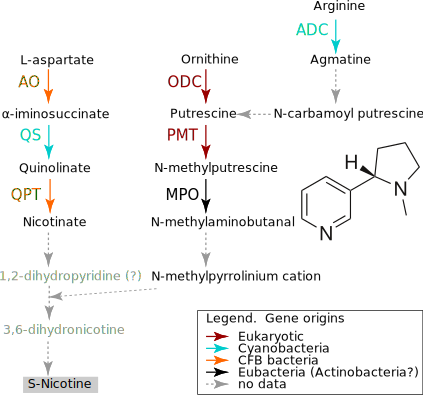
\includegraphics[width=.6\linewidth]{figures/pyridine_alkaloid_biosynthesis}
    \end{center}
    \caption{The nicotine biosynthetic pathway in tobacco consists of two
    sub-pathways, each representing a portion of the two rings of the nicotine
    molecule. The Jelesko lab analyzed each of the known enzymes to determine
    its evolutionary history. The result is a mosaic of putative most likely
    origins, illustrated in colors corresponding to closest known homologs as
    determined by rigorous phylogenetic analysis. \textit{Image courtesy of
    Prof.~John Jelesko.}}
    \label{fig:nicotine}
\end{figure}

Inspired by the intricate mosaic unveiled by their investigation into nicotine
biosynthesis, the Jelesko lab desired to expand their analyses to include
additional pathways. Their investigation of the nicotine pathway, however,
proved very time consuming, tedious, and prone to human error, as much of it
was a manual process. Additionally, Prof.~John Jelesko felt more sensitive
search by way of FASTA \cite{pearson_improved_1988} would prove helpful in
detecting homologous sequences more distantly related than BLAST could detect,
but unfortunately, NCBI does not provide FASTA search against their database,
due to its significantly costlier performance. Lastly, Prof.~Jelesko desired
to limit the search space to only sequences with full-genome sequencing
projects in NCBI, plus additional sequences from outside sources including
JGI. This would necessitate setting up a local database for storage of these
sequences and a means to integrate this database with homology search programs
in the FASTA and BLAST suites.

These challenges provided the motivation for our project:
\begin{enumerate}
    \item Collect all predicted protein sequences from NCBI belonging to
        organisms with whole genome sequencing projects either completed or
        undergoing completion.
    \item Collect additional sequences from JGI from pertinent genome
        projects.
    \item Organize these sequences into databases for storage and usable by
        the FASTA and BLAST suites of programs.
    \item Provide a user interface to homology searching against these
        sequences capable of easily being used by a bench biologist.
    \item Provide output from search programs and output sequences based on
        user selections from the search results in the format most useful for
        using the sequences for phylogenetic tree construction programs.
\end{enumerate}

Herein we describe our mostly successful attempts to meet these goals over the
semester by using high level tools to meet the short deadline, the
architecture behind the entire application we constructed, and our initial
results from deployment of the application.

\section{Methods (Yizhi Cai)}

Figure \ref{fig:The-workflow-of} shows the overall workflow of this
project. The whole project is database driven and composed of three
major components. The first component is Data acquisition, which needs
to fetch sequence data from NCBI and JGI using python scripts, and
integrate those data into a local MySQL database. The second major
component is user interfaces developed using Django framework, which
takes a protein sequence in FASTA format and user-specified parameters
to run homology search. Users can select hits of interests to download,
and this will link to the third major component of this project: the
user-specified output functionality. This component takes user-selected
GI numbers to query taxonomic information from the MySQL database
and provides users with output files in different formats.

\begin{figure}[btp]
    \begin{center}
        \includegraphics[width=0.95\linewidth]{figures/workflow.png}
    \end{center}
    \caption{\label{fig:The-workflow-of}The workflow of this project}
\end{figure}

\subsection{\label{sub:Data-Retrieval}Data Retrieval (Chris Lasher)}

Foremost, we were to retrieve all predicted protein sequences for all
organisms in NCBI's GenBank repository with completed or draft phase whole
genome sequencing projects, so that for later analyses, intron-exon
information for each gene could be guaranteed to be found, since the genes
were mapped to actual replicons (i.e., chromosomes and plasmids) rather than
fragmented scaffolds. Every organism that could be was to be included for
breadth of sequence diversity.

NCBI provides all whole-genome data via their FTP site, however, the directory
structure for the FTP site is somewhat troublesome to navigate in an automated
fashion. Chris Lasher developed a decently sophisticated Python script to
navigate the FTP site using a recursion algorithm modeled after the Python
standard library's \texttt{os.walk()} function, detect sequences in FASTA
format, and download them to local directories on the Jelesko lab server.

While we would have preferred to download more information-rich
representations of the sequences, such as the GenBank file format
representations, these more verbose formats were several times larger in size
than FASTA files, due to inclusion of entire nucleotide genome sequences. We
settled for retrieving the FASTA sequences, which only contained protein
sequence and limited information in the header lines of each record, instead,
given that later, functionality to look up the sequences via NCBI's EUtils
could be implemented.

These sequences were supplemented with current predictions from whole genome
plant projects hosted at NCBI that were unavailable via FTP, but available via
NCBI's Plant Genomes Central. The protein predictions for \textit{Glycine
max}, \textit{Medicago truncatula}, \textit{Oryza sativa}, \textit{Populus
trichocarpa}, \textit{Sorghum bicolor}, \textit{Vitis vinifera}, and
\textit{Zea mays} were manually downloaded and used to augment the collection.

Overall, we downloaded approximately 1.7 Gigabytes of data from NCBI,
amounting to greater than four million sequences.

Due to time constraints, no data from JGI was obtained, however, this should
be a fairly straightforward task for a technically proficient undergraduate.

\subsection{Data Integration (Chris Lasher)}

We developed a table in our database schema by which we could load in our
downloaded sequences and keep track of a minimal amount of desired
information, including download date, inferred genus and species information,
and annotations. Using Python scripts, we were able to massage the data into
formats acceptable for our MySQL database. Initial tests have shown that the
performance for queries over this table is acceptable, though certain queries
can take on the order of minutes. While this is not a problem for the Jelesko
lab, it should be taken into account should the application be considered for
opening to a greater community.

\subsection{Web Interface (Yizhi Cai)}

\begin{figure}[tbph]
    \begin{center}
        \includegraphics[width=1\linewidth]{figures/web_interface}
    \end{center}
    \caption{\label{fig:Web-interface}Web interface}
\end{figure}

Figure \ref{fig:Web-interface} outlines the web interface for running
FASTA search. There are three sections of this page. On the top of
the page, there is a sequence input diagram, which takes input sequence
in FASTA format. In the middle of the page, parameters can be specified
as necessary for running homology searches. These parameters include
the number of hits to return, the lower and upper e-value cutoffs,
substitution matrix, and the subject database to search against. Before
sending the input sequence and parameters to run search, it is important
to check the validity of those inputs. The validation includes non-empty
input of sequence, non-negative value of number of hits, and so on.
The validation increases the robustness of the entire web application.

\begin{figure}[tbp]
    \begin{center}
        \includegraphics[width=1\linewidth]{figures/Result_selection}
    \end{center}
    \caption{\label{fig:Homology-search-result}Homology search result}
\end{figure}

Once input sequence and user-specified parameters have been validated,
homology searches will be run in the backend. Outputs of the searches
will be interpreted using customized parser and Biopython modules
(see section \ref{sub:Integration-with-FASTA} for implementation
detail). The parsing result include the gi\_number, bit score and
e-value of each hit. And then we use the gi\_number to query the MySQL
database to pull out additional information, which includes accession,
geneus species, annotation and download date of each hit. Finally,
all the information is integrated and render in a nice representation
(see Figure \ref{fig:Homology-search-result}). Users can check certain
hits they are interested in to take a closer look. We also provide
checkall/uncheck all functionality by intergrating a java script.

Once a user specifies the hits to download, he/she will be redirected
to a download Page (see Figure \ref{fig:Users-selected-files}). The
implementation of the output functionality will be discussed in depth
in section \ref{sub:Output-Generation}. In the download page, there
are three files to be downloaded. The first file is the output file
generated by the homology search, which includes detail alignment
information of the search. The second file is a file containing all
selected sequences in FASTA format. And finally, the last file is
a file that maps internal-used Jelesko-ids to gi numbers.

The web site is built using Django, which is a Python driven framework
for rapid web development. Figure \ref{fig:Django-framework} shows
how Django works. The module of data model is used to interact with
various of databases, in our case, MySQL. Django provides a nice administrator
interface to add/delete entries in the database. The URL configuration
module is used to interpret input URL requests and map them to specific
functions in the view module. The view module is the core component
of the whole framework: it contains a list of functions to process
data from the data model according to the request from the URL module.
After the data has been processed, it will be render with HTML templates.

\begin{figure}[h]
\begin{center}
\includegraphics[width=0.6\linewidth]{figures/Django}
\end{center}

\caption{\label{fig:Django-framework}Django framework}

\end{figure}

\subsubsection{\label{sub:Integration-with-FASTA}Integration with FASTA and
BLAST (Yizhi Cai)}

\begin{figure}[tbp]
\begin{center}
\includegraphics[width=0.6\linewidth]{figures/Data_flow}
\end{center}

\caption{\label{fig:Integration-with-FASTA}Integration with FASTA and BLAST}

\end{figure}

Sequences database similarity search algorithms include two major
categories: algorithms based on dynamic programming and algorithms
based on heuristic algorithms. Widely used dynamic programming based
algorithms include Needleman-Wunsch algorithm and Smith-Waterman algorithm.
BLAST and FASTA are both based on heuristic algorithm. Generally speaking,
BLAST is faster than FASTA while FASTA outperforms BLAST in terms
of sensitivity. A benchmark comparison of BLAST and FASTA is described
in section \ref{fig:Benchmark-result}.

To enjoy the advantages of both, we need to integrate BLAST and FASTA.  After
the data retrieve and integration steps, we got a giant flat text file
containing 4 million sequence data. This text file has been imported as a
table in MySQL database, and also been converted into BLAST2 database format
using formatdb command. Both BLAST and FASTA search programs recognize the
BLAST2 format. For running BLAST search, we leveraged to use the BLAST module
of Biopython \citet{cock_biopython:_2009}, and also used the built-in parse to
process the output XML files.  Since there is no available modules for running
FASTA and parsing its output, we decided to use system call to run FASTA
program and save its output in the format of text file. Then a custom parser
has been implemented to process the output text file. The parsed output of
BLAST and FASTA includes a gi number, e-value and bit scores of each hit. Then
we developed scripts to query the MySQL database using the gi numbers. The
intergrated information finally is sent to the Django web interface.

\subsubsection{\label{sub:Output-Generation}Output Generation (Chris Lasher)}

\begin{figure}[tbp]
    \begin{center}
        \includegraphics[width=1\linewidth]{figures/User_selection}
    \end{center}
    \caption{\label{fig:Users-selected-files}Users selected files download}
\end{figure}


After running a homology search, the users can select among the hits returned
sequences that they would like to download for further analyses. (See Figure
\ref{fig:Users-selected-files}.) Typically,
these analyses involve constructing phylogenetic trees. The Jelesko lab uses
particular ID codes to facilitate readability of their phylogenetic trees.
Previously, translation of FASTA headers to these ``Jelesko IDs'' was handled
by a Perl script run manually. We implemented a simple version of this script
in Python using data stored in our database to help generate these Jelesko IDs
on the fly for each selection of a set of sequences users request from our
application.

Once the user has made his or her selections, the application presents the
user with a page at which he or she can download the results from his or her
search, a FASTA-formatted file containing the selected sequences with Jelesko
IDs as headers, and a mapping file that allows the user to back-translate from
the Jelesko IDs in their selections to GI numbers or equivalent unique
identifiers.  Alternatively, the application also presents the user with a
FASTA-formatted file that uses GI numbers or equivalent identifiers in the
headers of each record, should the user prefer those.

\section{Results (Yizhi Cai)}

In order to illustrate the application of this project, we used three
protein sequences (namely A622, NtNUP1 and NtMPO1) to benchmark three
homologous searches. Figure \ref{fig:Benchmark-result} presents the
benchmark result in terms of computation time and search sensitivity.
Searches are performed against the complete database, which contains
4 million sequences. The result suggests that both FASTA and Ssearch
are more computationally expensive than BLAST, but both obtain more
hits than BLAST. Also, we observe that with the close computational
time, Ssearch outperforms FASTA, especially in the case of A622.

\begin{figure}[tbph]
    \begin{center}
        \includegraphics[width=1\linewidth]{figures/Bench_mark_result}
    \end{center}
    \caption{\label{fig:Benchmark-result}Benchmark result}
\end{figure}

\section{Source code availability and further documentation (Chris Lasher)}

This paper does not cover actual deployment of the application we developed or
some of the more technical details. For these, we point the user to the GitHub
repository available at \\
\href{http://github.com/gotgenes/jelesko-lab-pathway-db/tree/master}{http://github.com/gotgenes/jelesko-lab-pathway-db/tree/master}

This page contains technical documentation, and also directs the user to
obtaining the source code, contained within a Git repository hosted at GitHub.

\section{Summaries and future work (Yizhi Cai)}

We began this project from scratch, and by the end of the semester
we have completed the project by accomplishing these tasks:
\begin{enumerate}
\item We have fetched more than 4 million sequences from NCBI.
\item We have developed custom parser for interpreting FASTA outputs, and
leveraged BioPython for data integration.
\item We have created MySQL, BLAST and FASTA databases for data storage.
\item We have built web interface for running BLAST, FASTA and Ssearch homology
searches.
\item We also have implemented user-specified output functionality.
\end{enumerate}
We envisage and would like to suggest a few future work for the continuation
of the project. First, additional sequence data should be retrieved
from NCBI. Second, we need to incorporate sequences from JGI and other
sources. Last, it will be helpful to save web searches for later reviewing.

\section{Author contributions}

Yizhi Cai created MySQL and BLAST2 databases for data storage, develped
web interface for running BLAST, FASTA and SSearch, implemented parsers
for parsing homology search results, wrote part of the final paper.

Chris Lasher developed the scripts to automate downloads from NCBI, all the
Django models to interface with the MySQL database, the views and logic behind
the web interface, the Python code to run the homology search programs, and the
code to generate output for user download. In conjunction with Alex Weisberg,
he deployed the production version of the site on the Jelesko lab server.
He wrote all technical documentation for the application.

\section{Acknowledgements}

Yizhi Cai and Chris Lasher would like to thank Prof.~John Jelesko for
overseeing the project and giving valuable supervision, Profs.~David Bevan and
Alexey Onufriev their instruction and additional input in the project and
presentations, and Alex Weisberg for his assistance with system administration
and deployment of the application on the production server.

\bibliographystyle{naturemag}
\bibliography{gbcbpaper}

\end{document}
